\section{Model Inversion Attacke}\label{sec:model_inversion}

Bei der Model Inversion Attacke, versucht ein Angreifer, durch bestimmte Eingaben in ein Modell, Rückschlüsse auf die Trainingsdaten von diesem zu ziehen. 
Dies kann so weit führen, dass einzelne Datensätze nachgebildet werden können \cite{P-3}. 

Fredrikson \etal \cite{P-3} zeigen anhand eines Gesichtserkennungsmodells, dass es möglich ist, das Bild einer Person zu rekonstruieren.
Dabei handelt es sich um einen sogenannten White-Box Angriff.
White-Box bedeutet, dass das Modell vollumfänglich in den Händen des Angreifers ist.
Dies ist beispielsweise der Fall, wenn ein Modell öffentlich geteilt wird.
Eine weitere Voraussetzung ist, dass die zu rekonstruierende Person von dem anzugreifenden Modell klassifiziert werden kann, folglich auch Bilder dieser Person in den Trainingsdaten vorhanden sind.
Abbildung \ref{fig:mi_attacke} zeigt, wie sehr das rekonstruierte Bild (links) dem Originalbild (rechts) ähnelt.

\begin{figure}[!htb]
    \centering
    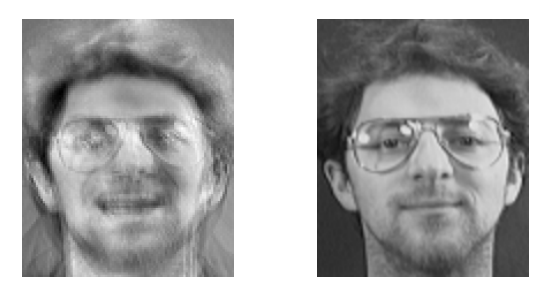
\includegraphics[width=8cm]{figures/mi_attack}
    \caption{Rekonstruktion eines Bildes \cite{P-3}}
    \label{fig:mi_attacke}
\end{figure} 

Der Angriff, auch Reconstruction Attacke genannt, wird durch einen iterativen Algorithmus durchgeführt.
Zu Beginn wird ein initiales Bild, als Startbild gesetzt. 
Hat der Angreifer Hintergrundwissen zu den Daten, so kann er das initiale Bild ähnlich zu dem Zielbild setzen, ansonsten kann es mit festgelegten konstanten Werten oder zufälligen Werten initialisiert werden. 
In jedem Schritt des Algorithmus wird dieses Bild durch das Modell inferiert und anschließend der Wert einer Verlustfunktion bestimmt.
Der Wert dieser ist, sofern das Modell nicht mehr Details zur Vorhersage angibt, lediglich der Wert 1 minus die Wahrscheinlichkeit, auch Confidence Score genannt, ob es sich bei dem eingegebenen Bild um die gesuchte Klasse, auch Label genannt, handelt.
Konkret bedeutet dies, wenn das Bild bereits die zu rekonstruierende Person zeigt, ist der Confidence Score des Labels der Person nahe 1 und damit der Wert der Verlustfunktion nahe 0.
Der Wert der Verlustfunktion kann nun durch das Modell abgeleitet werden und ergibt somit Gradienten für das Bild.
Dies gleicht dem Backpropagation Schritt des Trainings eines neuronalen Netzes, mit dem Unterschied, dass hier das Bild wie ein Teil des Modells behandelt wird und für dieses ebenfalls Gradienten berechnet werden.
Diese Gradienten werden genutzt, um das Bild entgegengesetzt dieser Gradienten anzupassen, sodass der Wert der Verlustfunktion sinkt.
Zusätzlich nutzen die Autoren einen Autoencoder, welcher das angepasste Bild in jedem Schritt harmonisiert und hochskaliert.
Bei diesem Autoencoder handelt es sich um ein neuronales Netz, welches einen Input (hier ein Bild) in einen Vektor mit niedrigerem Rang transformiert und anschließend wieder in einen Vektor mit dem gleichen Rang wie der des Inputs transformiert.
Input und Output eines Autoencoders haben somit den gleichen Rang, hier wird also ein Bild zu einem anderen Bild der gleichen Größe transformiert.
Der Teil des Autoencoders, welcher das Eingabebild in einen Vektor mit niedrigerem Rang transformiert, wird Encoder genannt. 
Der Teil des Autoencoders, welcher das Hochskalieren übernimmt, heißt Decoder.
Zum Training des Autoencoders werden Bilder genutzt, wobei der Input auch gleich dem gewünschten Output entspricht. 
Somit lernt ein Autoencoder, aus einem Bild das gleiche Bild zu erzeugen, jedoch mit der Einschränkung, dass der Vektor innerhalb des Modells einen niedrigen Rang hat.
Folglich ist das erzeugte Bild nicht exakt identisch zu dem eingegebenen Bild.
Der Autoencoder von Fredrikson \etal \cite{P-3} weist jedoch die Besonderheit auf, dass die Eingabebilder verrauscht werden und die gewünschten Ausgabebilder gleich bleiben.
Ziel dadurch ist es, dass der trainierte Autoencoder genutzt werden kann, um unscharfe Bilder zu möglichst scharfen Bildern zu transformieren.
Mit diesem Autoencoder soll also das rekonstruierte Bild nach jeder Iteration schärfer werden und damit näher an dem ursprünglichen Bild liegen.
Die Reconstruction Attacke läuft so lange, bis die maximal konfigurierte Anzahl an Schritten erreicht wird, der Wert der Verlustfunktion einen bestimmten Wert unterschreitet oder sich eine definierte Anzahl an Schritten der Wert der Verlustfunktion nicht reduziert.

Zhang \etal \cite{P-4} erweitern diesen Angriff, indem die Qualität des Autoencoders verbessert wird. 
Der Autoencoder wird nicht nur auf verschwommenen Bildern trainiert, sondern zusätzlich noch auf Bilder, bei welchen jeweils nur ein Bildausschnitt maskiert wird.
Eine weitere Verbesserung besteht darin, zusätzlich ein Modell zu nutzen, welches reale Bilder von synthetischen Bildern unterscheiden soll.
Dieses Konstrukt entspricht dem Diskriminator eines Generative Adversarial Networks \cite{P-86}.
Als Input nutzt dieser Diskriminator Bilder, welche von dem Autoencoder generiert wurden.
Der Wert einer Verlustfunktion des Outputs des Diskriminators kann dabei nicht nur durch den Diskriminator selbst backpropagiert werden, sondern zusätzlich auch noch durch den Autoencoder.
Dies sorgt dafür, dass der Autoencoder ergänzend versucht, möglichst realistische Bilder zu erzeugen.
Mithilfe der zusätzlichen Trainingsdaten und des Diskriminators, wird der Autoencoder verbessert, wodurch die Qualität der einzelnen Bilder erhöht wird und folglich auch die Qualität des rekonstruierten Bildes steigt.
Der restliche Angriff erfolgt simultan zu der bereits beschriebenen Vorgehensweise.
Zhang \etal \cite{P-4} zeigen einen zusätzlichen Angriffsvektor, bei dem ein Angreifer bereits Teile eines Bildes hat. 
Dabei kann es sich um eine verschwommene Version des originalen Bildes handeln, oder um ein Bild, bei dem ein Teil beispielsweise mit einem schwarzen Balken zensiert wird.
Da der Autoencoder zusätzlich mit diesen Fällen trainiert wurde, ist es möglich, die fehlenden Informationen eines Bildes zu ergänzen.


